\FloatBarrier
\section{Silicon process and physical design}\label{sec:process}

\subsection{Process technology}
\ac{1} is built in a 3 nm-class gate-all-around process with nanosheet channels, 16 nm wide and
5 nm thick, stacked three high with a 45 nm contacted gate pitch and a 24 nm metal pitch. The
standard-cell library is 6-track with four threshold voltages. The backend has 12 front-side metal
layers with the top layers at 56 nm pitch, and three backside layers for power delivery.

Backside power delivery is not optional at this design point. A 0.75 V, 80 A part in a two-slot
card needs a supply grid with roughly half the resistance of a front-side grid, and the front side
does not have the tracks to spare: 15 layers would have been needed, and the routing congestion
model (Fig.~\ref{fig:physical}(c)) shows the design already at 94\% utilisation on M7--M9. Moving
power to the back frees the front for signal, cuts the static IR drop from 62 mV to 48 mV, and
reduces via resistance from 1.8 to 0.9 $\Omega$.

\begin{figure}[t]
\centering
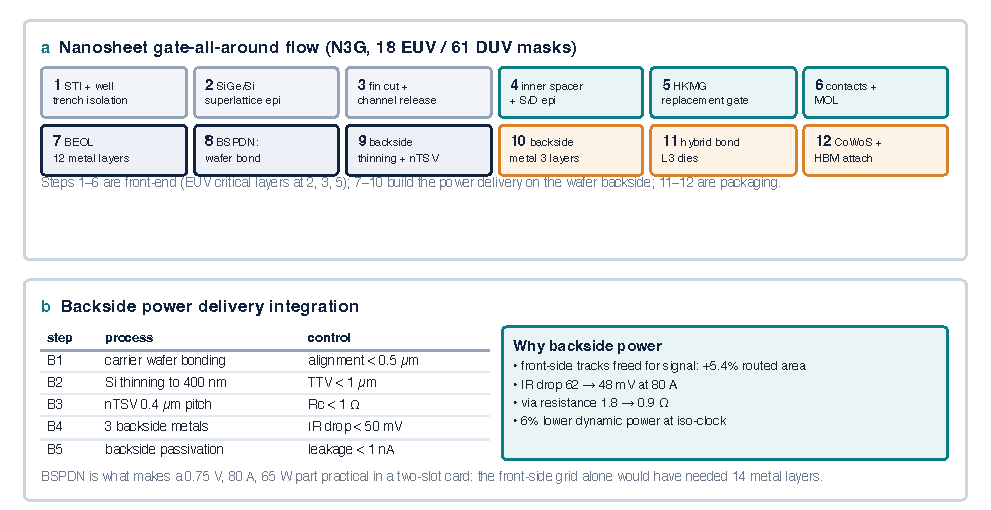
\includegraphics[width=\linewidth]{fig19_process}
\caption{Process integration. (a) Twelve-step nanosheet flow from shallow-trench isolation to
CoWoS attach; 18 EUV and 61 DUV masks. (b) Backside power delivery sequence and its process
controls.}
\label{fig:process}
\end{figure}

\subsection{Interconnect and power grid}
The front-side stack is split into local (M1--M4, 24--32 nm), intermediate (M5--M8, 32--40 nm) and
global (M9--M12, 56 nm) layers. Halo and NoC links are routed on M9--M12 at twice the minimum
width for electromigration margin; the tile SRAM bitlines and the SFU datapath stay on M2--M5. The
backside stack carries VDD and VSS with a 0.4 $\mu$m nTSV pitch, which is what allows the 80 A
delivery without a front-side mesh.

\begin{figure}[t]
\centering
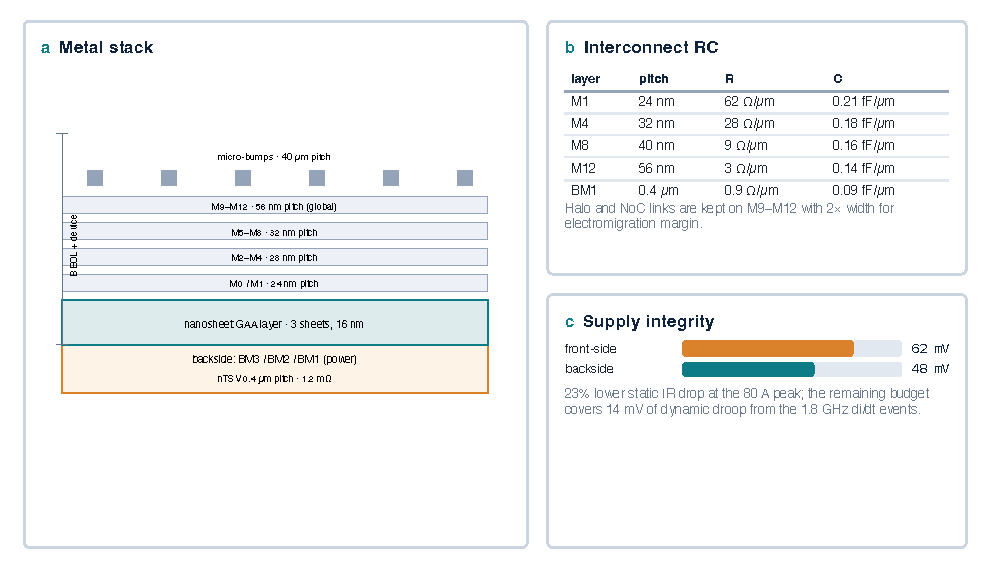
\includegraphics[width=\linewidth]{fig20_beol}
\caption{Backend and supply. (a) Metal stack with the device layer and the backside power layers.
(b) Resistance and capacitance by layer. (c) Static IR drop, front-side against backside.}
\label{fig:beol}
\end{figure}

\subsection{Floorplan and physical implementation}
The floorplan follows the logical organisation almost literally: eight clusters in a 4$\times$2
array around an L3/NoC spine, HBM PHYs on the bottom edge next to the interposer microbumps, SerDes
on the top edge next to the card edge connector. The 64 AVTs are placed as identical hard macros to
keep the clock tree shallow and the SRAM bank pattern regular. Placement density peaks at 88\% in
the cluster array and falls to 62\% at the SerDes, which is the usual shape for a die with a large
digital core and high-speed I/O.

The clock tree has 14 levels and a measured skew of 9 ps at the slow corner, achieved by matching
the 64 tile macros and using a spine-and-mesh distribution over the cluster array. Dynamic
frequency scaling is per cluster, with a 12-cycle handshake; the runtime can drop an idle cluster
to 0.55 V without disturbing its neighbours.

\begin{figure}[t]
\centering
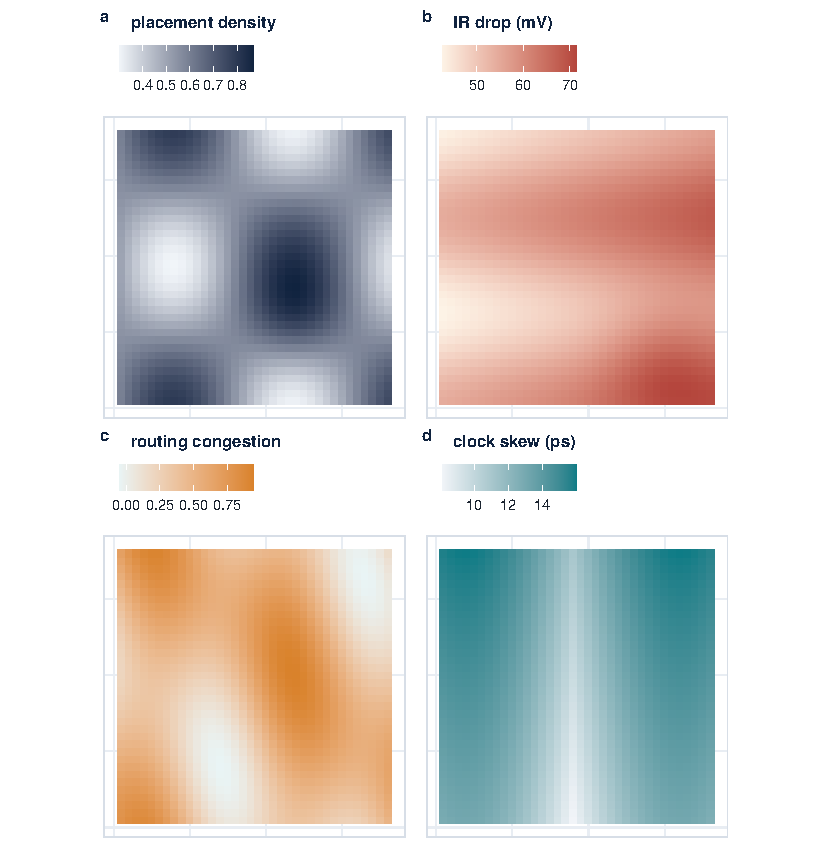
\includegraphics[width=\linewidth]{fig21_physical}
\caption{Physical-design estimates. (a) Placement density. (b) Static IR drop at the 80 A peak.
(c) Routing congestion; M7--M9 are the critical layers. (d) Clock skew across the die. These are
model-based estimates from the floorplan, not sign-off results.}
\label{fig:physical}
\end{figure}

\subsection{Package and board}
The package is 55 $\times$ 45 mm on a 2.5D silicon-bridge interposer of two reticles. The compute
die and the two HBM stacks sit on the interposer; the two 64 MB L3 dies are hybrid-bonded directly
on top of the compute die with a 6 $\mu$m pitch, which gives 128 MB at 0.40 pJ/B and avoids a
third interposer hop. The card is dual-slot and 267 mm long, powered from the slot alone: at 65 W
the 12 V rail draws 5.5 A, well inside the 5.5 A per-slot limit with margin.

\begin{figure}[t]
\centering
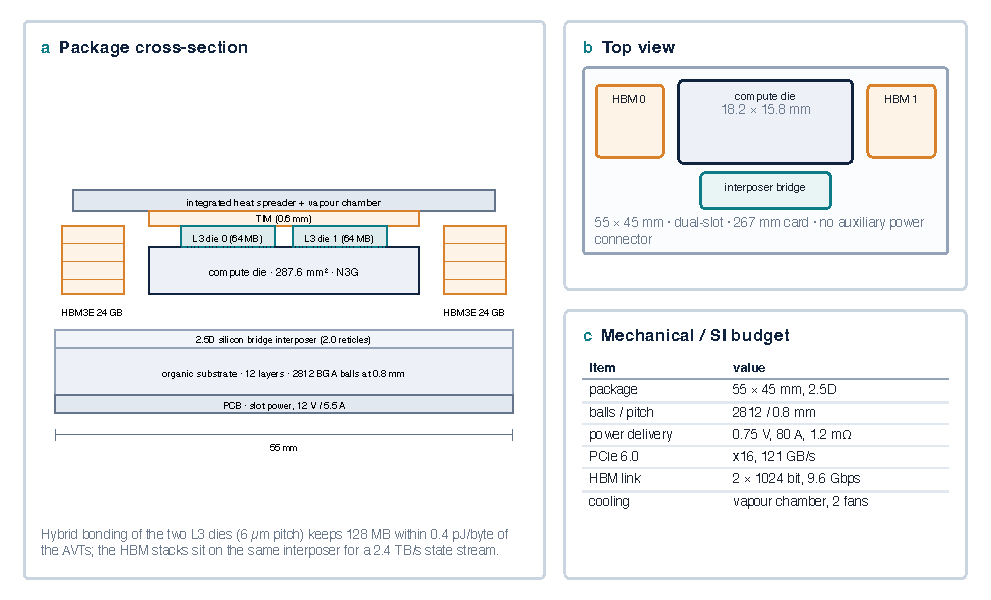
\includegraphics[width=\linewidth]{fig18_package}
\caption{Package. (a) Cross-section: heat spreader, TIM, hybrid-bonded L3 dies, compute die,
interposer, substrate and PCB. (b) Top view. (c) Mechanical and signal-integrity budget.}
\label{fig:package}
\end{figure}

\subsection{Power and thermal}
The thermal design targets a 35 $^\circ$C ambient and a 95 $^\circ$C junction limit. The network is
modelled as three resistances --- junction-to-lid 0.18 K/W, lid-to-heatsink 0.28 K/W,
heatsink-to-ambient 0.19 K/W --- for a total of 0.65 K/W. At the 65 W TDP the steady-state junction
is \ACTjSteady$^\circ$C; during the W1 workload at 57.1 W it is 74 $^\circ$C. A step from idle to
full load reaches 76 $^\circ$C in about 90 s, which is slow enough that the fan controller can
track it without overshoot.

\begin{figure}[t]
\centering
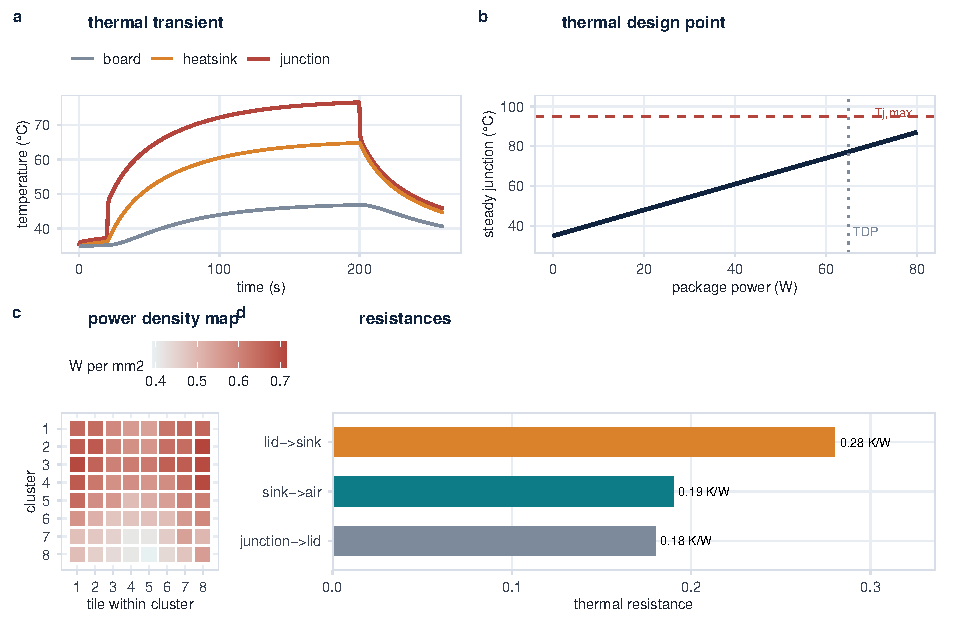
\includegraphics[width=\linewidth]{fig16_thermal}
\caption{Thermal behaviour. (a) Transient response to a 65 W step from idle. (b) Steady-state
junction temperature against power, with the TDP and the 95 $^\circ$C limit marked. (c) Modelled
power density across the 64 tiles. (d) Thermal resistance budget.}
\label{fig:thermal}
\end{figure}

The voltage--frequency curve is modelled with an $\alpha$-power law and a temperature-dependent
leakage term. The efficiency mode (1.05 GHz at 0.55 V) sits at the minimum of the energy-per-FLOP
curve; the performance mode (1.8 GHz at 0.75 V) sits at the knee of the frequency curve. The
runtime chooses between them from the job's deadline, which is why the software stack exposes a
``time budget'' parameter rather than a clock frequency.

\begin{figure}[t]
\centering
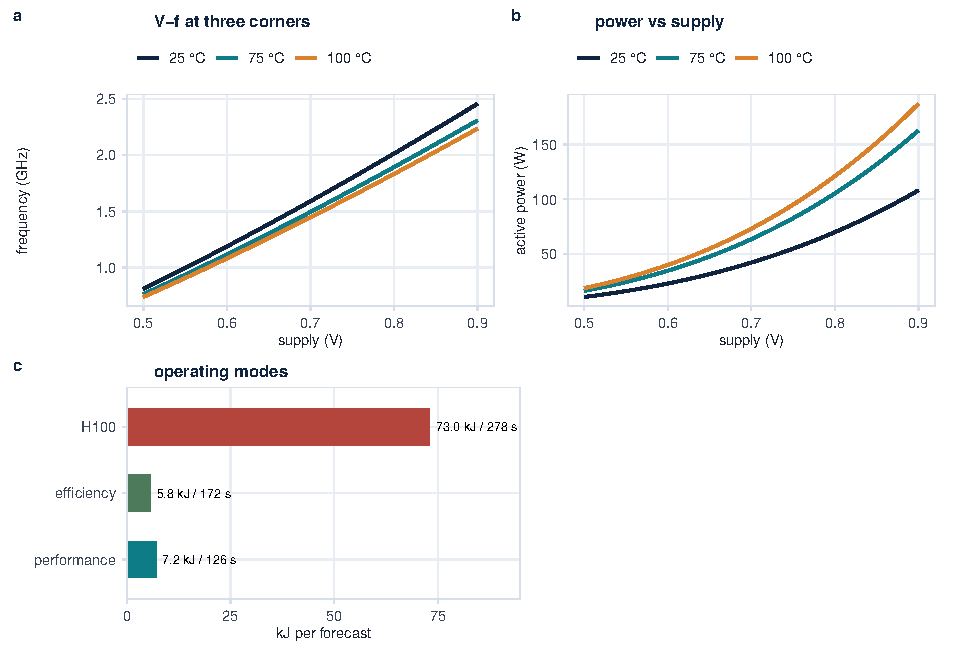
\includegraphics[width=\linewidth]{fig17_voltage}
\caption{Voltage and frequency. (a) Frequency against supply at three junction temperatures.
(b) Active power. (c) The two operating modes against the H100 on the energy--time plane.}
\label{fig:voltage}
\end{figure}
